\documentclass[12pt,a4paper]{article}

\makeatletter
	% ---------------------- %
% -- GENERAL SETTINGS -- %
% ---------------------- %

\usepackage[
	top    = 2cm,
	bottom = 2cm,
	left   = 1.5cm,
	right  = 1.5cm
]{geometry}

\usepackage[utf8]{inputenc}
\usepackage[T1]{fontenc}
\usepackage{ucs}

\usepackage[french]{babel,varioref}

\usepackage{color}
\usepackage{hyperref}
\hypersetup{
    colorlinks,
    citecolor = black,
    filecolor = black,
    linkcolor = black,
    urlcolor  = black
}
\usepackage[numbered]{bookmark}

\usepackage{enumitem}
\usepackage{multicol}
\usepackage{longtable}
\usepackage{makecell}

\setlength{\parindent}{0cm}
\setlist{noitemsep}



% --------------- %
% -- TOC & Co. -- %
% --------------- %

\usepackage[raggedright]{titlesec}

%\renewcommand\thechapter{\Alph{chapter}.}
\renewcommand\thesection{\Roman{section}.}
\renewcommand\thesubsection{\arabic{subsection}.}
\renewcommand\thesubsubsection{\roman{subsubsection}.}


\titleformat{\paragraph}[hang]{\normalfont\normalsize\bfseries}{\theparagraph}{1em}{}
\titlespacing*{\paragraph}{0pt}{3.25ex plus 1ex minus .2ex}{0.5em}


% Source
%    * https://tex.stackexchange.com/a/558025/6880
\usepackage{tocbasic}[2020/07/22]% needs KOMA-Script version 3.31

\DeclareTOCStyleEntries[
    raggedentrytext,
    linefill = \hfill,
    indent   = 0pt,
    dynindent,
    numwidth = 0pt,
    numsep   = 1ex,
    dynnumwidth
]{tocline}{
	chapter,
	section,
	subsection,
	subsubsection,
	paragraph,
	subparagraph
}

\DeclareTOCStyleEntry[indentfollows = chapter]{tocline}{section}



% ----------- %
% -- TOOLS -- %
% ----------- %

\usepackage{ifplatform}
\usepackage{ifthen}
\usepackage{macroenvsign}
\usepackage{pgffor}



% ------------------------- %
% -- SPECIAL FORMATTINGS -- %
% ------------------------- %

\usepackage{amsthm}

\usepackage{tcolorbox}


% -- LISTINGS -- %

%\tcbuselibrary{listingsutf8}
\tcbuselibrary{minted, breakable}

\newtcblisting{latexex}{%
    breakable,%
    sharp corners,%
    left   = 1mm, right = 1mm,%
    bottom = 1mm, top   = 1mm,%
    %colupper = red!75!blue,%
    listing side text
}

\newtcbinputlisting{\inputlatexex}[2][]{%
    listing file={#2},%
    breakable,
    sharp corners,%
    left   = 1mm, right = 1mm,%
    bottom = 1mm, top   = 1mm,%
    %colupper = red!75!blue,%
    listing side text
}


\newtcblisting{latexex-flat}{%
    breakable,
    sharp corners,%
    left   = 1mm, right = 1mm,%
    bottom = 1mm, top   = 1mm,%
    %colupper = red!75!blue,%
}

\newtcbinputlisting{\inputlatexexflat}[2][]{%
    listing file={#2},%
    breakable,
    sharp corners,%
    left   = 1mm, right = 1mm,%
    bottom = 1mm, top   = 1mm,%
    %colupper = red!75!blue,%
}


\newtcblisting{latexex-alone}{%
    breakable,
    sharp corners,%
    left   = 1mm, right = 1mm,%
    bottom = 1mm, top   = 1mm,%
    %colupper = red!75!blue,%
    listing only
}

\newtcbinputlisting{\inputlatexexalone}[2][]{%
    listing file={#2},%
    breakable,
    sharp corners,%
    left   = 1mm, right = 1mm,%
    bottom = 1mm, top   = 1mm,%
    %colupper = red!75!blue,%
    listing only
}


\newcommand\inputlatexexcodeafter[1]{%
    \begin{center}
        \input{#1}
    \end{center}

    \vspace{-.5em}
    
    Le rendu précédent a été obtenu via le code suivant.
    
    \inputlatexexalone{#1}
}


\newcommand\inputlatexexcodebefore[1]{%
    \inputlatexexalone{#1}
    \vspace{-.75em}
    \begin{center}
        \textit{\footnotesize Rendu du code précédent}
        
        \medskip
        
        \input{#1}
    \end{center}
}


% -- REMARK -- %

\theoremstyle{definition}
\newtheorem*{remark}{Remarque}


% -- EXAMPLE -- %

\newcounter{paraexample}[subsubsection]

\newcommand\@newexample@abstract[2]{%
    \paragraph{%
        #1%
        \if\relax\detokenize{#2}\relax\else {} -- #2\fi%
    }%
}

\newcommand\newparaexample{\@ifstar{\@newparaexample@star}{\@newparaexample@no@star}}

\newcommand\@newparaexample@no@star[1]{%
    \refstepcounter{paraexample}%
    \@newexample@abstract{Exemple \theparaexample}{#1}%
}

\newcommand\@newparaexample@star[1]{%
    \@newexample@abstract{Exemple}{#1}%
}


% -- CHANGE LOG -- %

\newcommand\topic{\@ifstar{\@topic@star}{\@topic@no@star}}

\newcommand\@topic@no@star[1]{%
    \textbf{\textsc{#1}.}%
}

\newcommand\@topic@star[1]{%
    \textbf{\textsc{#1} :}%
}


% -- ABOUT MACROS & Co. -- %

\newcommand\env[1]{\texttt{#1}}
\newcommand\macro[1]{\env{\textbackslash{}#1}}

\newcommand\separation{
    \medskip
    \hfill\rule{0.5\textwidth}{0.75pt}\hfill
    \medskip
}


\newcommand\extraspace{
    \vspace{0.25em}
}


\newcommand\whyprefix[2]{%
    \textbf{\prefix{#1}}-#2%
}

\newcommand\mwhyprefix[2]{%
    \texttt{#1 = #1-#2}%
}

\newcommand\prefix[1]{%
    \texttt{#1}%
}


\newcommand\inenglish{\@ifstar{\@inenglish@star}{\@inenglish@no@star}}

\newcommand\@inenglish@star[1]{%
    \emph{\og #1 \fg}%
}

\newcommand\@inenglish@no@star[1]{%
    \@inenglish@star{#1} en anglais%
}


\newcommand\ascii{\texttt{ASCII}}

	
	\usepackage{01-env}
\makeatother


\begin{document}

\section{Écriture \texttt{pseudo verbatim}}

\newparaexample{Avec toutes les options}

\inputlatexex{examples/pseudo-verb-all-options.extra.tex}


Voici comment s'utilise chacune des options.

\begin{enumerate}
	\item \verb#title# permet de donner un titre \textbf{si un cadre est utilisé}. Un titre vide sera ignoré. Par défaut cette option est de valeur vide.

	\item \verb#frame# demande d'ajouter un cadre autour du contenu.

	\item \verb#center# sert à centrer le contenu.

	\item \verb#scale# permet de donner un coefficient d'échelle à appliquer à la largeur de la ligne. Par défaut cette option vaut \verb#1#.
\end{enumerate}


% ---------------------- %


\newparaexample{Ajouter juste un cadre}

\inputlatexex{examples/pseudo-verb-just-frame.extra.tex}


% ---------------------- %


\newparaexample{Sans option, un piège à éviter !}

Voici un 1\ier{} exemple montrant qu'il faut faire attention quand on ne veut pas indiquer d'option.
Il semble naturel d'omettre \verb#[]# avant le contenu mais ce qui suit met en lumière un petit problème quand on veut garder tous les espaces  initiaux du contenu.
 
\inputlatexex{examples/pseudo-verb-no-option-bad.extra.tex}


Ce qui précède est tout à fait normal puisque \LaTeX\ ignore les espaces au début du contenu lorsqu'il commence par chercher un crochet ouvrant indiquant une option du point de vue de l'environnement.
Une fois que \LaTeX\ tombe sur un caractère autre que \verb#[# , l'option par défaut est utilisée mais malheureusement les espaces initiaux ont été mangés, ils sont perdus à tout jamais.
Pour éviter le problème précédent, il suffit d'utiliser une option vide via \verb#[]# comme ci-dessous.
 
\inputlatexex{examples/pseudo-verb-no-option-good.extra.tex}


Le code suivant montre que \LaTeX\ peut voir une option là où l'on voudrait indiquer un contenu. Bien que l'option ne soit pas correcte, elle est silencieusement ignorée en coulisse. Ceci explique que ce qui est entre des crochets ci-dessous ne soit pas affiché.

\inputlatexex{examples/pseudo-verb-pseudo-option-error.extra.tex}


De nouveau la solution consiste à utiliser une option vide \verb#[]# comme le montre l'exemple ci-après.

\inputlatexex{examples/pseudo-verb-pseudo-option-error-good.extra.tex}


% ---------------------- %


\newparaexample{Macros interprétées}

Dans ce document, \macro{squaremacro} a été définie par \verb#\newcommand\squaremacro{$x^2$}#.
Le code ci-après montre que l'environnement \env{pseudoverb} interprète les macros
\footnote{
	Ceci permet de définir assez facilement des contenus indentés de type langage de programmation via la définition de macros de mise en forme des mots-clés.
}.

\newcommand\squaremacro{$x^2$}

\inputlatexex{examples/pseudo-verb-env-with-macro.extra.tex}


% ---------------------- %


\newparaexample{Du contenu sur plusieurs pages}

Même avec un cadre un contenu pourra se trouver sur des pages successives.

\begin{figure}[hbt!]
	\centering
	\frame{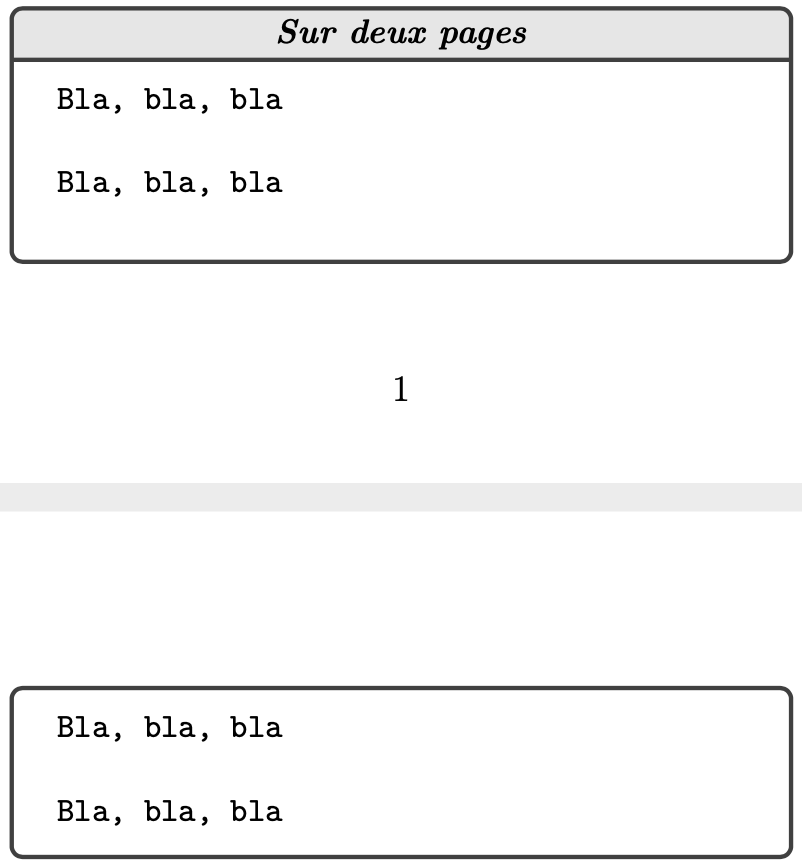
\includegraphics[scale = .5]{images/pseudo-verb-broken[fr].png}}
\end{figure}


% ---------------------- %


\section{Fiches techniques}

\IDenv[o]{pseudoverb}{1}

\IDoption{} on utilise un système clé/valeur.
\begin{enumerate}
	\item \verb#title# est le titre du cadre.
	      Par défaut \verb#title = {}#.

	\item \verb#frame# demande d'ajouter un cadre.

	\item \verb#center# sert à centrer le contenu.

	\item \verb#scale# donne le coefficient multiplicatif à appliquer à la largeur de la ligne.
	      Par défaut \verb#scale = 1#.
\end{enumerate}

\end{document}
